\section{LIMS}

 \begin{figure}[h]
 \centering
 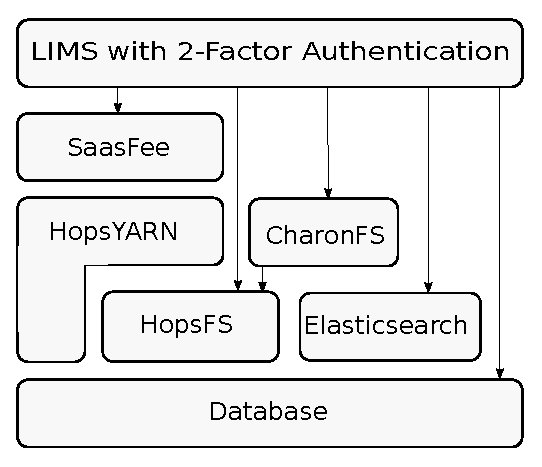
\includegraphics[scale=0.8]{./imgs/stack.eps}
 % stack.eps: 0x0 pixel, 300dpi, 0.00x0.00 cm, bb=0 -1 805 312
 \caption{BiobankCloud Architecture}
 \label{fig:lim}
\end{figure}


BiobankCloud introduces \textbf{DataSets} as a new abstraction to Hadoop, where a DataSet consists of a related group of directories, files, and extended metadata. DataSets can be indexed and searched and are the basic unit of data management in BiobankCloud; all user-generated files or directories belong to a single DataSet. In Biobanking, a sample collection would be a typical example of a DataSet.  To allow for access control of users to DataSets, which is not inherent in the DataSet concept, we introduce the notion of \textbf{Studies}. A Study is a grouping of researchers and DataSets , see figure \ref{fig:studies}. 
% The basic user roles we provide reflect the European Data Protection Directive, with a DataOwner (data controller) and a DataScientist (data processer). DataSets can be shared between Studies (when the necessary security, legal, and ethical conditions for sharing are in place).  In BiobankCloud, we use the access control mechanism of HopsFS to implement the Study- and DataSet-based authorization model. 
% Roles are defined and privileges are enforced in HopsFS.
\begin{figure}[h]
 \centering
 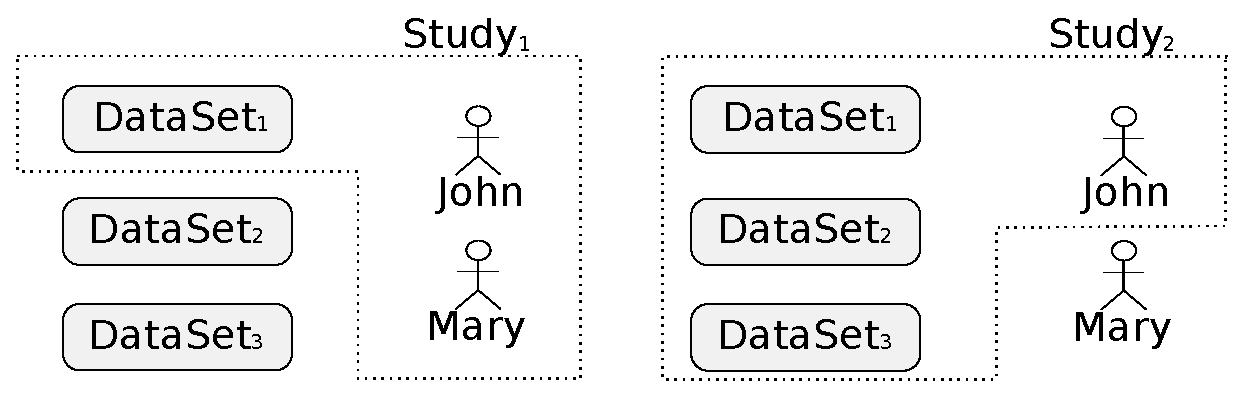
\includegraphics[scale=0.6]{./imgs/projects-as-groupings1.eps}
 % projects-as-groupings1.eps: 0x0 pixel, 300dpi, 0.00x0.00 cm, bb=0 207 582 382
\caption{Study1 has two Users and one DataSet, while Study2 has one User and three DataSets.}
\label{fig:studies}
\end{figure}
